\documentclass[12pt]{article}
\usepackage[utf8]{inputenc}
\usepackage{geometry}
\geometry{letterpaper, margin=0.25in}
\usepackage{graphicx} 
\usepackage{parskip}
\usepackage{booktabs}
\usepackage{array} 
\usepackage{paralist} 
\usepackage{verbatim}
\usepackage{subfig}
\usepackage{fancyhdr}
\usepackage{sectsty}
\usepackage[shortlabels]{enumitem}

\pagestyle{fancy}
\renewcommand{\headrulewidth}{0pt} 
\lhead{}\chead{}\rhead{}
\lfoot{}\cfoot{\thepage}\rfoot{}

%%% ToC (table of contents) APPEARANCE
\usepackage[nottoc,notlof,notlot]{tocbibind} 
\usepackage[titles,subfigure]{tocloft}
\renewcommand{\cftsecfont}{\rmfamily\mdseries\upshape}
\renewcommand{\cftsecpagefont}{\rmfamily\mdseries\upshape} %

\usepackage{amsmath}
\usepackage{amssymb}
\usepackage{mathtools}
\usepackage{empheq}
\usepackage{xcolor}
\usepackage{bbm}
\usepackage{tikz}
\usepackage{pgfplots}
\usepackage{tikz-cd}
\pgfplotsset{compat=1.18}
\usetikzlibrary{intersections, decorations.markings}
\tikzset{
    marking along/.style n args={2}{
        decoration={
                markings, 
                mark=at position #1 with {\arrow{#2}}
        },
        postaction={decorate}
        },
    marking along/.default={0.5}{>}
}

\newcommand{\ans}[1]{\boxed{\text{#1}}}
\newcommand{\vecs}[1]{\langle #1\rangle}
\renewcommand{\hat}[1]{\widehat{#1}}

\renewcommand{\P}{\mathbb{P}}
\newcommand{\R}{\mathbb{R}}
\newcommand{\E}{\mathbb{E}}
\newcommand{\Z}{\mathbb{Z}}
\newcommand{\N}{\mathbb{N}}
\newcommand{\Q}{\mathbb{Q}}
\newcommand{\C}{\mathbb{C}}

\newcommand{\ind}{\mathbbm{1}}
\newcommand{\qed}{\quad \blacksquare}

\newcommand{\brak}[1]{\left\langle #1 \right\rangle}
\newcommand{\bra}[1]{\left\langle #1 \right\vert}
\newcommand{\ket}[1]{\left\vert #1 \right\rangle}

\newcommand{\abs}[1]{\left\vert #1 \right\vert}
\newcommand{\mfX}{\mathfrak{X}}
\newcommand{\ep}{\varepsilon}

\newcommand{\Ec}{\mathcal{E}}
\newcommand{\A}{\mathcal{A}}
\newcommand{\F}{\mathcal{F}}
\newcommand{\Cc}{\mathcal{C}}
\newcommand{\B}{\mathcal{B}}
\newcommand{\M}{\mathcal{M}}
\newcommand{\X}{\chi}
\renewcommand{\L}{\mathcal{L}}

\newcommand{\sub}{\subseteq}
\newcommand{\st}{\text{ s.t. }}
\newcommand{\card}{\text{card }}
\renewcommand{\div}{\vspace*{10pt}\hrule\vspace*{10pt}}
\newcommand{\surj}{\twoheadrightarrow}
\newcommand{\inj}{\hookrightarrow}
\newcommand{\biject}{\hookrightarrow \hspace{-8pt} \rightarrow}
\renewcommand{\bar}[1]{\overline{#1}}
\newcommand{\overcirc}[1]{\overset{\circ}{#1}}
\newcommand{\diam}{\text{diam }}

\renewcommand{\Re}{\text{Re}\,}
\renewcommand{\Im}{\text{Im}\,}
\newcommand{\sign}{\text{sign}\,}

\newcommand*{\tbf}[1]{\ifmmode\mathbf{#1}\else\textbf{#1}\fi}

\usepackage{tcolorbox}
\tcbuselibrary{breakable, skins}
\tcbset{enhanced}
\newenvironment*{tbox}[2][gray]{
    \begin{tcolorbox}[
        parbox=false,
        colback=#1!5!white,
        colframe=#1!75!black,
        breakable,
        title={#2}
    ]}
    {\end{tcolorbox}}

\newenvironment*{exercise}[1][red]{
    \begin{tcolorbox}[
        parbox=false,
        colback=#1!5!white,
        colframe=#1!75!black,
        breakable
    ]}
    {\end{tcolorbox}}

\newenvironment*{proof}[1][blue]{
\begin{tcolorbox}[
    parbox=false,
    colback=#1!5!white,
    colframe=#1!75!black,
    breakable
]}
{\end{tcolorbox}}

\colorlet{mygreen}{green!50!teal}


\title{APMA 1360 - Homework 5}
\author{Milan Capoor}
\date{28 February 2025}

\begin{document}
\maketitle

\section*{Problem 1}

Please state the existence and uniqueness theorem for solutions of differential equations. Make sure you include all assumptions and the conclusions in a concise, clear, and complete fashion.

\color{blue}
Let $f \in C^1$ and $u_0 \in \R$. Then $\dot u = f(u)$ with $u(0) = u_0$ has a unique solution on some interval around $t = 0$.
\color{black}

%%%%%%%%%%%%%%%%%%%%%%%%%%%%%%%%

\pagebreak
\section*{Problem 2}

Determine analytically the fixed points and their stability of the differential equation
\[
    \dot{x} = (x-1)(x-2).
\]

\color{blue}
Let $f(x) = (x-1)(x-2)$.

\[f(x) = 0 \implies x = \{1, 2\}\]

Further,
\[f(x) = x^2 -3x + 2 \implies f'(x) = 2x -3 \implies \begin{cases}
        x = 1 & \implies f'(1) = -1< 0 \implies \text{stable}   \\
        x = 2 & \implies f'(2) = 2 > 0 \implies \text{unstable}
    \end{cases}\]
\color{black}


%%%%%%%%%%%%%%%%%%%%%%%%%%%%%%%%

\pagebreak
\section*{Problem 3}

\begin{enumerate}[(a)]
    \item Sketch the bifurcation diagram of a supercritical pitchfork bifurcation.

          \begin{center}
              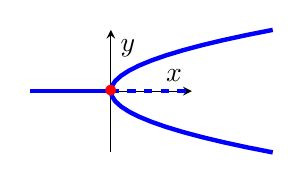
\begin{tikzpicture}
                  \begin{axis}[
                          width=0.3\textwidth,
                          axis lines=middle,
                          no markers,
                          xtick=\empty,
                          ytick=\empty,
                          clip=false,
                          xlabel={$x$},
                          ylabel={$y$},
                          domain=-2:2,
                          ymin=-2, ymax=2,
                          xmin= -2, xmax=2,
                          view = {0}{90}
                      ]
                      \addplot[blue, ultra thick, domain=-2:0] {0};
                      \addplot[blue, ultra thick, dashed, domain=0:2] {0};

                      \addplot[blue, ultra thick, domain=-2:2] ({x^2}, {x});

                      \node[red] at (0,0) {$\bullet$};
                  \end{axis}
              \end{tikzpicture}
          \end{center}

    \item For which of the following three differential equations on the line would it be possible to have a pitchfork bifurcation? Explain your answers. Do \underline{not} calculate any bifurcation points.
          \begin{enumerate}[(i)]
              \item \quad $\dot{x} = \mu x - x^3$

                    \color{blue}
                    Yes.
                    \begin{itemize}
                        \item $f(-x, \mu) = -\mu x + x^3 = -f(x, \mu)$
                        \item $f_x(0, 0) = 0$
                        \item $f_{x\mu}(0, 0) = 1 \neq 0$
                        \item $f_{xxx}(0, 0) = 6 \neq 0$
                    \end{itemize}
                    \color{black}

              \item \quad $\dot{x} = \mu x + 10 x^2$

                    \color{blue}
                    No. $f(-x, \mu) = -\mu x + 10x^2 \neq -f(x, \mu)$.
                    \color{black}

              \item \quad $\dot{x} = 1 + \mu x - x^3$

                    \color{blue}
                    No. $f(-x, \mu) = 1 -\mu x + x^3 \neq -f(x, \mu)$
                    \color{black}
          \end{enumerate}
\end{enumerate}

%%%%%%%%%%%%%%%%%%%%%%%%%%%%%%%%

\pagebreak
\section*{Problem 4}

Consider the following three potential bifurcation diagrams for a differential equation $\dot{x}=f(x,\mu)$ on the line, where stable or unstable fixed points are drawn as solid or dashed curves, respectively.

For each diagram, circle all bifurcation points in the $(\mu,x)$-plane and classify them as saddle-node, transcritical, subcritical pitchfork or supercritical pitchfork, or argue why the resulting diagram is impossible. Be careful and take your time.

\begin{center}
    \begin{tikzpicture}
        \node at (0,0) {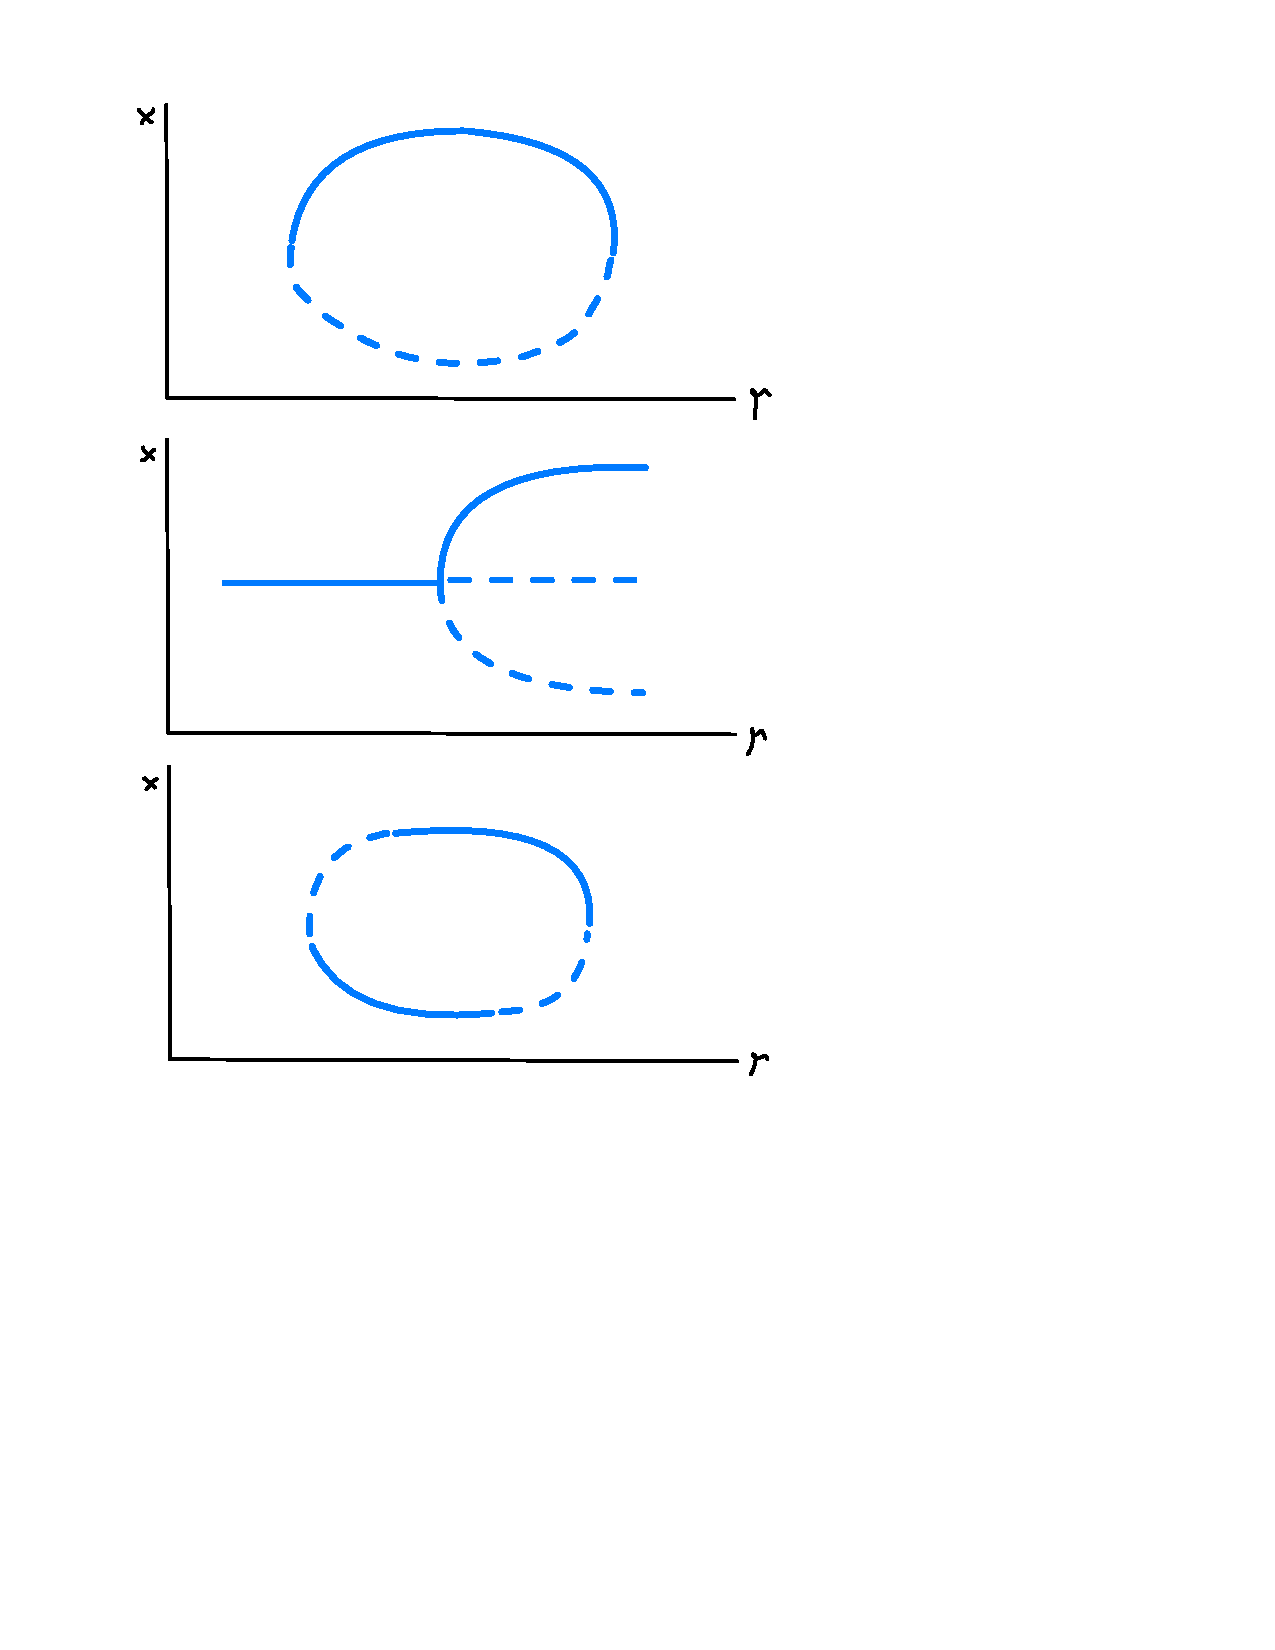
\includegraphics[scale=0.8]{Assignment_Figure_7.pdf}};

        %% 1 %%
        \node[red, scale=2] at (2.1, 4.4) {$\bullet$};
        \node[red, scale=2] at (-2.2, 4.4) {$\bullet$};
        \node [red, scale=2] at (6, 4.5) {$\bullet$};
        \node at (7.5, 4.5) {Saddle-node};

        %% 2 %%
        \node at (8, 0) {\parbox{2in}{Impossible. We would need to have a stable point between the lower branches of the pitchfork}};

        %% 3 %% 

        \node[red, scale=2] at (1.8, -4.4) {$\bullet$};
        \node[red, scale=2] at (-2, -4.8) {$\bullet$};
        \node[red, scale=2] at (0.5, -5.8) {$\bullet$};
        \node[red, scale=2] at (-1, -3.45) {$\bullet$};

        \node at (8, -4.5) {\parbox{2in}{Impossible. We would expect to see a saddle point at the center of the loop to account for the two stable regions and the two unstable regions.}};

    \end{tikzpicture}

\end{center}

%%%%%%%%%%%%%%%%%%%%%%%%%%%%%%%%

\pagebreak
\section*{Problem 5}

Find and classify all equilibria and the bifurcation points of the differential equation
\[
    \dot{x} = x (\mu - 2 - x)
\]
and sketch the resulting bifurcation diagram. In the bifurcation diagram, indicate stable and unstable fixed points by solid and dashed lines, respectively, and sketch the direction of other representative solutions using arrows.

\color{blue}
Let $f(x, \mu) = x(\mu - 2 - x)$.

We can check:
\begin{align*}
    f(0, \mu)      & = 0             \\
    f_x(0, 2)      & = 2 - 2 - 0 = 0 \\
    f_{x\mu}(0, 2) & = 1 \neq 0      \\
    f_{xx}(0, 2)   & = -2 \neq 0
\end{align*}
so we have a transcritical bifurcation at $(0, 2)$.

Now, we want to examine stability for varying $\mu$. We have phase diagrams:

\begin{center}
    \color{black}
    \begin{tabular}{ccc}
        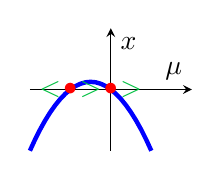
\begin{tikzpicture}
            \begin{axis}[
                    width=0.3\textwidth,
                    axis lines=middle,
                    no markers,
                    xtick=\empty,
                    ytick=\empty,
                    clip=false,
                    xlabel={$\mu$},
                    ylabel={$x$},
                    domain=-2:2,
                    ymin=-2, ymax=2,
                    xmin= -2, xmax=2,
                    view = {0}{90}
                ]
                \addplot[blue, ultra thick, domain=-2:1] {-x^2 + (1 - 2)*x};

                \node[red] at (0,0) {$\bullet$};
                \node[red] at (-1,0) {$\bullet$};

                \node[mygreen] at (-1.5, 0) {$<$};
                \node[mygreen] at (-0.5, 0) {$>$};
                \node[mygreen] at (0.5, 0) { $>$};

            \end{axis}
        \end{tikzpicture} &
        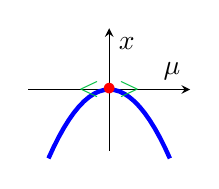
\begin{tikzpicture}
            \begin{axis}[
                    width=0.3\textwidth,
                    axis lines=middle,
                    no markers,
                    xtick=\empty,
                    ytick=\empty,
                    clip=false,
                    xlabel={$\mu$},
                    ylabel={$x$},
                    domain=-2:2,
                    ymin=-2, ymax=2,
                    xmin= -2, xmax=2,
                    view = {0}{90}
                ]
                \addplot[blue, ultra thick, domain=-1.5:1.5] {-x^2 + (2 - 2)*x};

                \node[red] at (0,0) {$\bullet$};

                \node[mygreen] at (-0.5, 0) {$<$};
                \node[mygreen] at (0.5, 0) {$>$};
            \end{axis}
        \end{tikzpicture} &
        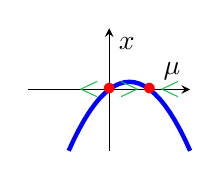
\begin{tikzpicture}
            \begin{axis}[
                    width=0.3\textwidth,
                    axis lines=middle,
                    no markers,
                    xtick=\empty,
                    ytick=\empty,
                    clip=false,
                    xlabel={$\mu$},
                    ylabel={$x$},
                    domain=-2:2,
                    ymin=-2, ymax=2,
                    xmin= -2, xmax=2,
                    view = {0}{90}
                ]
                \addplot[blue, ultra thick, domain=-1:2] {-x^2 + (3 - 2)*x};

                \node[red] at (0,0) {$\bullet$};
                \node[red] at (1,0) {$\bullet$};

                \node[mygreen] at (-0.5, 0) {$<$};
                \node[mygreen] at (0.5, 0) {$>$};
                \node[mygreen] at (1.5, 0) {$<$};
            \end{axis}
        \end{tikzpicture}                          \\
        $\mu < 2$                 & $\mu = 2$ & $\mu > 2$
    \end{tabular}
\end{center}

which yields the bifurcation diagram:
\begin{center}
    \color{black}
    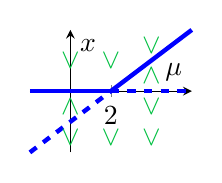
\begin{tikzpicture}
        \begin{axis}[
                width=0.3\textwidth,
                axis lines=middle,
                no markers,
                xtick={1},
                xticklabels={$2$},
                ytick=\empty,
                clip=false,
                xlabel={$\mu$},
                ylabel={$x$},
                domain=-2:2,
                ymin=-2, ymax=2,
                xmin= -1, xmax=3,
                view = {0}{90}
            ]
            \addplot[blue, ultra thick, domain=-1:1] {0};
            \addplot[blue, ultra thick, dashed, domain=1:3] {0};

            \addplot[blue, ultra thick, dashed, domain=-1:1] {x - 1};
            \addplot[blue, ultra thick, domain=1:3] {x - 1};

            \node[mygreen] at (0, 1) {\rotatebox{180}{$\wedge$}};
            \node[mygreen] at (1, 1) {\rotatebox{180}{$\wedge$}};
            \node[mygreen] at (0, -0.5) {$\wedge$};
            \node[mygreen] at (2, -0.5) {\rotatebox{180}{$\wedge$}};
            \node[mygreen] at (2, 0.5) {$\wedge$};
            \node[mygreen] at (0, -1.5) {\rotatebox{180}{$\wedge$}};
            \node[mygreen] at (1, -1.5) {\rotatebox{180}{$\wedge$}};
            \node[mygreen] at (2, -1.5) {\rotatebox{180}{$\wedge$}};
            \node[mygreen] at (2, 1.5) {\rotatebox{180}{$\wedge$}};

        \end{axis}
    \end{tikzpicture}
\end{center}


\color{black}
%%%%%%%%%%%%%%%%%%%%%%%%%%%%%%%%

\pagebreak
\section*{Problem 6}

Consider the system
\begin{eqnarray*}
    \dot{x} & = & y-2x \\
    \dot{y} & = & \mu+x^2-y.
\end{eqnarray*}
Use the nullclines to graphically find and classify all bifurcations that occur as $\mu$ varies. You do \textbf{not} need to find analytical values for the bifurcation points, determine the stability of the equilibria, or draw the phase portrait or bifurcation diagram.

\color{blue}
Let $f(x, y) = y - 2x$ and $g(x, y) = \mu + x^2 - y$.

Then the nullcline of $f$ is
\[\{(x, y): f = 0\} = \{(x, 2x): x \in \R\}\]

and the nullcline of $g$ is
\[\{(x, y): g = 0\} = \{(x, x^2 + \mu): x \in \R\}\]

We have three situations:

\begin{center}
    \color{black}
    \begin{tabular}{ccc}
        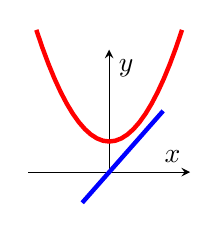
\begin{tikzpicture}
            \begin{axis}[
                    width=0.3\textwidth,
                    axis lines=middle,
                    no markers,
                    xtick=\empty,
                    ytick=\empty,
                    clip=false,
                    xlabel={$x$},
                    ylabel={$y$},
                    domain=0:4,
                    ymin=0, ymax=8,
                    xmin= -3, xmax=3,
                    view = {0}{90}
                ]
                \addplot[blue, ultra thick, domain=-1:2] {2*x};
                \addplot[red, ultra thick, domain=-2.7:2.7] {x^2 + 2};
            \end{axis}
        \end{tikzpicture} &
        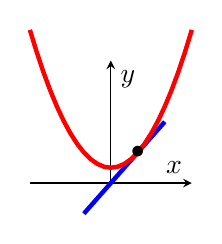
\begin{tikzpicture}
            \begin{axis}[
                    width=0.3\textwidth,
                    axis lines=middle,
                    no markers,
                    xtick=\empty,
                    ytick=\empty,
                    clip=false,
                    xlabel={$x$},
                    ylabel={$y$},
                    domain=0:4,
                    ymin=0, ymax=8,
                    xmin= -3, xmax=3,
                    view = {0}{90}
                ]
                \addplot[blue, ultra thick, domain=-1:2] {2*x};
                \addplot[red, ultra thick, domain=-3:3] {x^2+1};

                \node at (1,2) {$\bullet$};

            \end{axis}
        \end{tikzpicture} &
        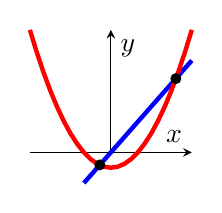
\begin{tikzpicture}
            \begin{axis}[
                    width=0.3\textwidth,
                    axis lines=middle,
                    no markers,
                    xtick=\empty,
                    ytick=\empty,
                    clip=false,
                    xlabel={$x$},
                    ylabel={$y$},
                    domain=0:6,
                    ymin=0, ymax=8,
                    xmin= -3, xmax=3,
                    view = {0}{90}
                ]
                \addplot[name path=b, blue, ultra thick, domain=-1:3] {2*x};
                \addplot[name path=r, red, ultra thick, domain=-3:3] {x^2 - 1};

                \fill [name intersections={of=b and r, total=\t}]
                \foreach \s in {1,...,\t}{(intersection-\s) circle (2pt)};

            \end{axis}
        \end{tikzpicture}                          \\
        $\mu =1$                   & $\mu > 1$ & $\mu < 1$
    \end{tabular}

\end{center}

Hence we have a saddle-node bifurcation at $\mu = 1$.

\color{black}

%%%%%%%%%%%%%%%%%%%%%%%%%%%%%%%%

\pagebreak
\section*{Problem 7}

Show that the solutions of the equation
\[
    4 y - x^2 + x^3 - y^4 - 3 = 0
\]
near $(1,1)$ are of the form $(x,y)=(g(y),y)$ where $y$ can be chosen arbitrarily near $1$.

\color{blue}
Let $f(x, y) = 4y - x^2 + x^3 - y^4 - 3$.

Certainly, $f \in C^{\infty}$. Hence, by the IFT, it suffices to show that $f(1, 1) = 0$ and $f_x(1, 1) \neq 0$.

Observe:
\begin{align*}
    f(1, 1)   & = 4 - 1 + 1 - 1 - 3 = 0                    \\
    f_x(1, 1) & = [-2x + 3x^2]_{(1, 1)} = -2 + 3 = 1\neq 0
\end{align*}

Since $f$ satisfies the conditions of the IFT, we know $\exists g \in C^{\infty}$ such that $f(x, y) = 0 \iff x = g(y)$ near $(1, 1)$, i.e. $f(x, y) = 0 \iff (x, y) = (g(y), y)$ near $(1, 1) \qed$.
\color{black}


%%%%%%%%%%%%%%%%%%%%%%%%%%%%%%%%%%%%%%%%%%%%%%%%%%%%%%%%%%%%%%%%%%%%%%%%%%%%


\end{document}